\documentclass[twocolumn,10pt]{article}

\usepackage[a4paper,hmargin=1.5cm,vmargin=2.5cm,]{geometry}
\setlength{\columnsep}{0.7cm}
\usepackage{amsmath}
\usepackage{graphicx}
\usepackage[utf8]{inputenc}
\usepackage{hyperref}
\urlstyle{same} % no tt font for URLs

\usepackage{natbib}
\bibliographystyle{genome_research}
%\setcitestyle{aysep={}} 

\usepackage[dvipsnames]{xcolor}
\hypersetup{
    colorlinks,
    linkcolor={blue!50!black},
    citecolor={blue!50!black},
    urlcolor={blue!50!black}
}
\renewcommand{\dbltopfraction}{0.7}
\renewcommand{\textfraction}{0.2}

\begin{document}

\setcounter{secnumdepth}{0}

\twocolumn[{%
\centering
\textbf{\Large Analysing single-cell bisulfite sequencing data with scbs}

Lukas P.~M. Kremer\textsuperscript{1,2}, Leonie Küchenhoff\textsuperscript{1,2}, Santiago Cerrizuela\textsuperscript{2}, ..., Ana Martin-Villalba\textsuperscript{2}, Simon Anders\textsuperscript{1}\\
{\footnotesize \textsuperscript{1} BioQuant, University of Heidelberg, Germany}\\
{\footnotesize \textsuperscript{2} Molecular Neurobiology, German Cancer Research Center (DKFZ), Heidelberg, Germany}
\vspace{1.5ex}

March 2022
\vspace{6ex}
}]

\section{Abstract}

[...]

\section{Introduction}

Sequencing-based assays with single-cell resolution have offered new means to understand the differences between the cells making up a sample. Single-cell RNA sequencing (scRNA-seq) techniques have matured at great pace in recent years, and methods to study chromatin are rapidly catching up. Of special interest here is DNA methylation, i.e., the methylation of bases in the DNA, because DNA methylation patterns are passed on to daughter cells in cell division. Especially in mammals, such methylation chiefly occurs at cytosine bases that are immediately after followed by guanine bases, so-called CpG sites. 

To detect CpG methylation by sequencing, bisulfite conversion is commonly employed: treatment of DNA with bisulfite causes unmethylated cytosine bases to be deaminated to uracil, which is paired with thymine in subsequent PCR. Therefore, unmethylated CpGs are read as TG in sequencing of bisulfite-converted DNA while only methylated CpG is correctly read as CG \citep{Frommer_1992}. Such so-called bisulfite sequencing has been used for bulk samples since long, and methods for bisulfite sequencing with single-cell resolution (scBS) were recently developed \citep{Smallwood_2014} and are increasingly used.

CpG dinocleotides are underrepresented in eukaryotic genomes (due to their vulnerability to mutation by conversion to TpG due to accidental deamination), and the majority of existing CpG sites are methylated. Presence or absence of the methyl group at CpG sites is believed to have effect on gene regulation, with methylation inhibiting transcription. Methylating DNA during differentiation is therefore conjectured to be an important mechanism to silence genome regions that are not needed in the target lineage. One important application of single-cell bisulfite sequencing (scBS) therefore lies in the study of differentiation processes.

In the present paper, we discuss strategies to analyze scBS data, suggest improvement to current approaches, show their value in a benchmark, and present software to perform the improved analysis methods.

\subsection{Standard approach}

We start by briefly reviewing the standard approach of analyzing single-cell \emph{RNA}-Seq data, and how this approach is typically adapted to the case of single-cell DNA methylation data.

The starting point in scRNA-Seq is a matrix of UMI counts (i.e. of counts of distinct RNA molecules), one row for each cell and one column for each gene. As a first step towards assigning cell types or states to cells, one needs to establish which cells are similar to each other, and to this end, find a way to quantify the distance (i.e., dissimilarity) between any two given cells' transcriptional profile. A standard approach, used with minor variation in virtually all recent research and automated by popular software such as Seurat \citep{Hao_2021} or ScanPy \citep{Wolf_2018}, is as follows: One first accounts for cell-to-cell variation in sequencing depth by dividing each UMI count by the respective cell's total UMI count, then transforms to a homoskedastic scale by taking the logarithm. In order to avoid matrix elements with zero count to be transformed to minus infinity, one typically adds a very small ``pseudocount'' (often $10^{-5}$) to the normalized fractions before taking the logarithm. Now, one could use Euclidean distances of these vectors  of logarithmized fractions as dissimilarity score. However, these scores would be exceedingly noisy due to the strong Poisson noise introduced by the many genes with very low counts. Therefore, one performs a principal component analysis (PCA), keeping only the top few (typically, 20 to 50) components. As Poisson noise is uncorrelated between genes, it will average out in the top principal components. Therefore, Euclidean distances between these ``PCA space'' vectors provide a robust dissimilarity score, which can subsequently be used as input to methods like t-SNE and UMAP, which provide a two-dimensional representation of the data. The PCA space representation is furthermore used for clustering (assigning cells to groups by similarity) and trajectory finding (identifying elongated manifolds in PCA space and assigning cells to quasi-1D positions along them).

\begin{figure}
	\framebox[\columnwidth]{
		\begin{minipage}[c][3.5cm]{\columnwidth}
			\centering Figure
		\end{minipage}
	}
	\caption{\small UMAP representations of the single-cell bisulfite data of XXX et al., calculated \textbf{(A)} using conventional preprocessing and \textbf{(B)} using the approach described here.}
	\label{umaps}
\end{figure}


This procedure is commonly adapted when working with single-cell DNA-methylation data, so that all the tools used in scRNA-Seq downstream of the PCA step can be used. The question is therefore how to construct a suitable matrix as input for the PCA. A simple and popular approach is to tile the genome into windows of, say, 100 kB size, and calculate for each cell the average methylation of the DNA within each window. To this end, we identify all CpG sites in the window for which we have coverage with at least one read and can hence call the CpG to be either unmethylated or methylated in the cell. Then we denote as average DNA methylation of this window in a given cell the proportion of observed CpG sites in the window have been found to be methylated. This yields a matrix, with one row for each cell and one column for each window from the genome tiling, comprising numbers (methylation fractions) between 0 and 1. This matrix is now subjected to PCA.

As an example, we will us in this paper data from XX et al., who have performed scBS on [...] and analysed their data in the manner just described. Figure \ref{umaps}A shows a UMAP plot, derived from our re-analysis of the data, using a tiling of the genome into windows of size 100 kb. As one can see, the approach is suitable to see clear structure in the data, observe ...

Nevertheless, this analysis strategy has substantial room for improvement, as we will discuss next. Here, we discuss the proposed improvements only qualitatively. For the mathematical details, please see the Methods section. 

\begin{figure*}
	A\\
    \begin{center}
        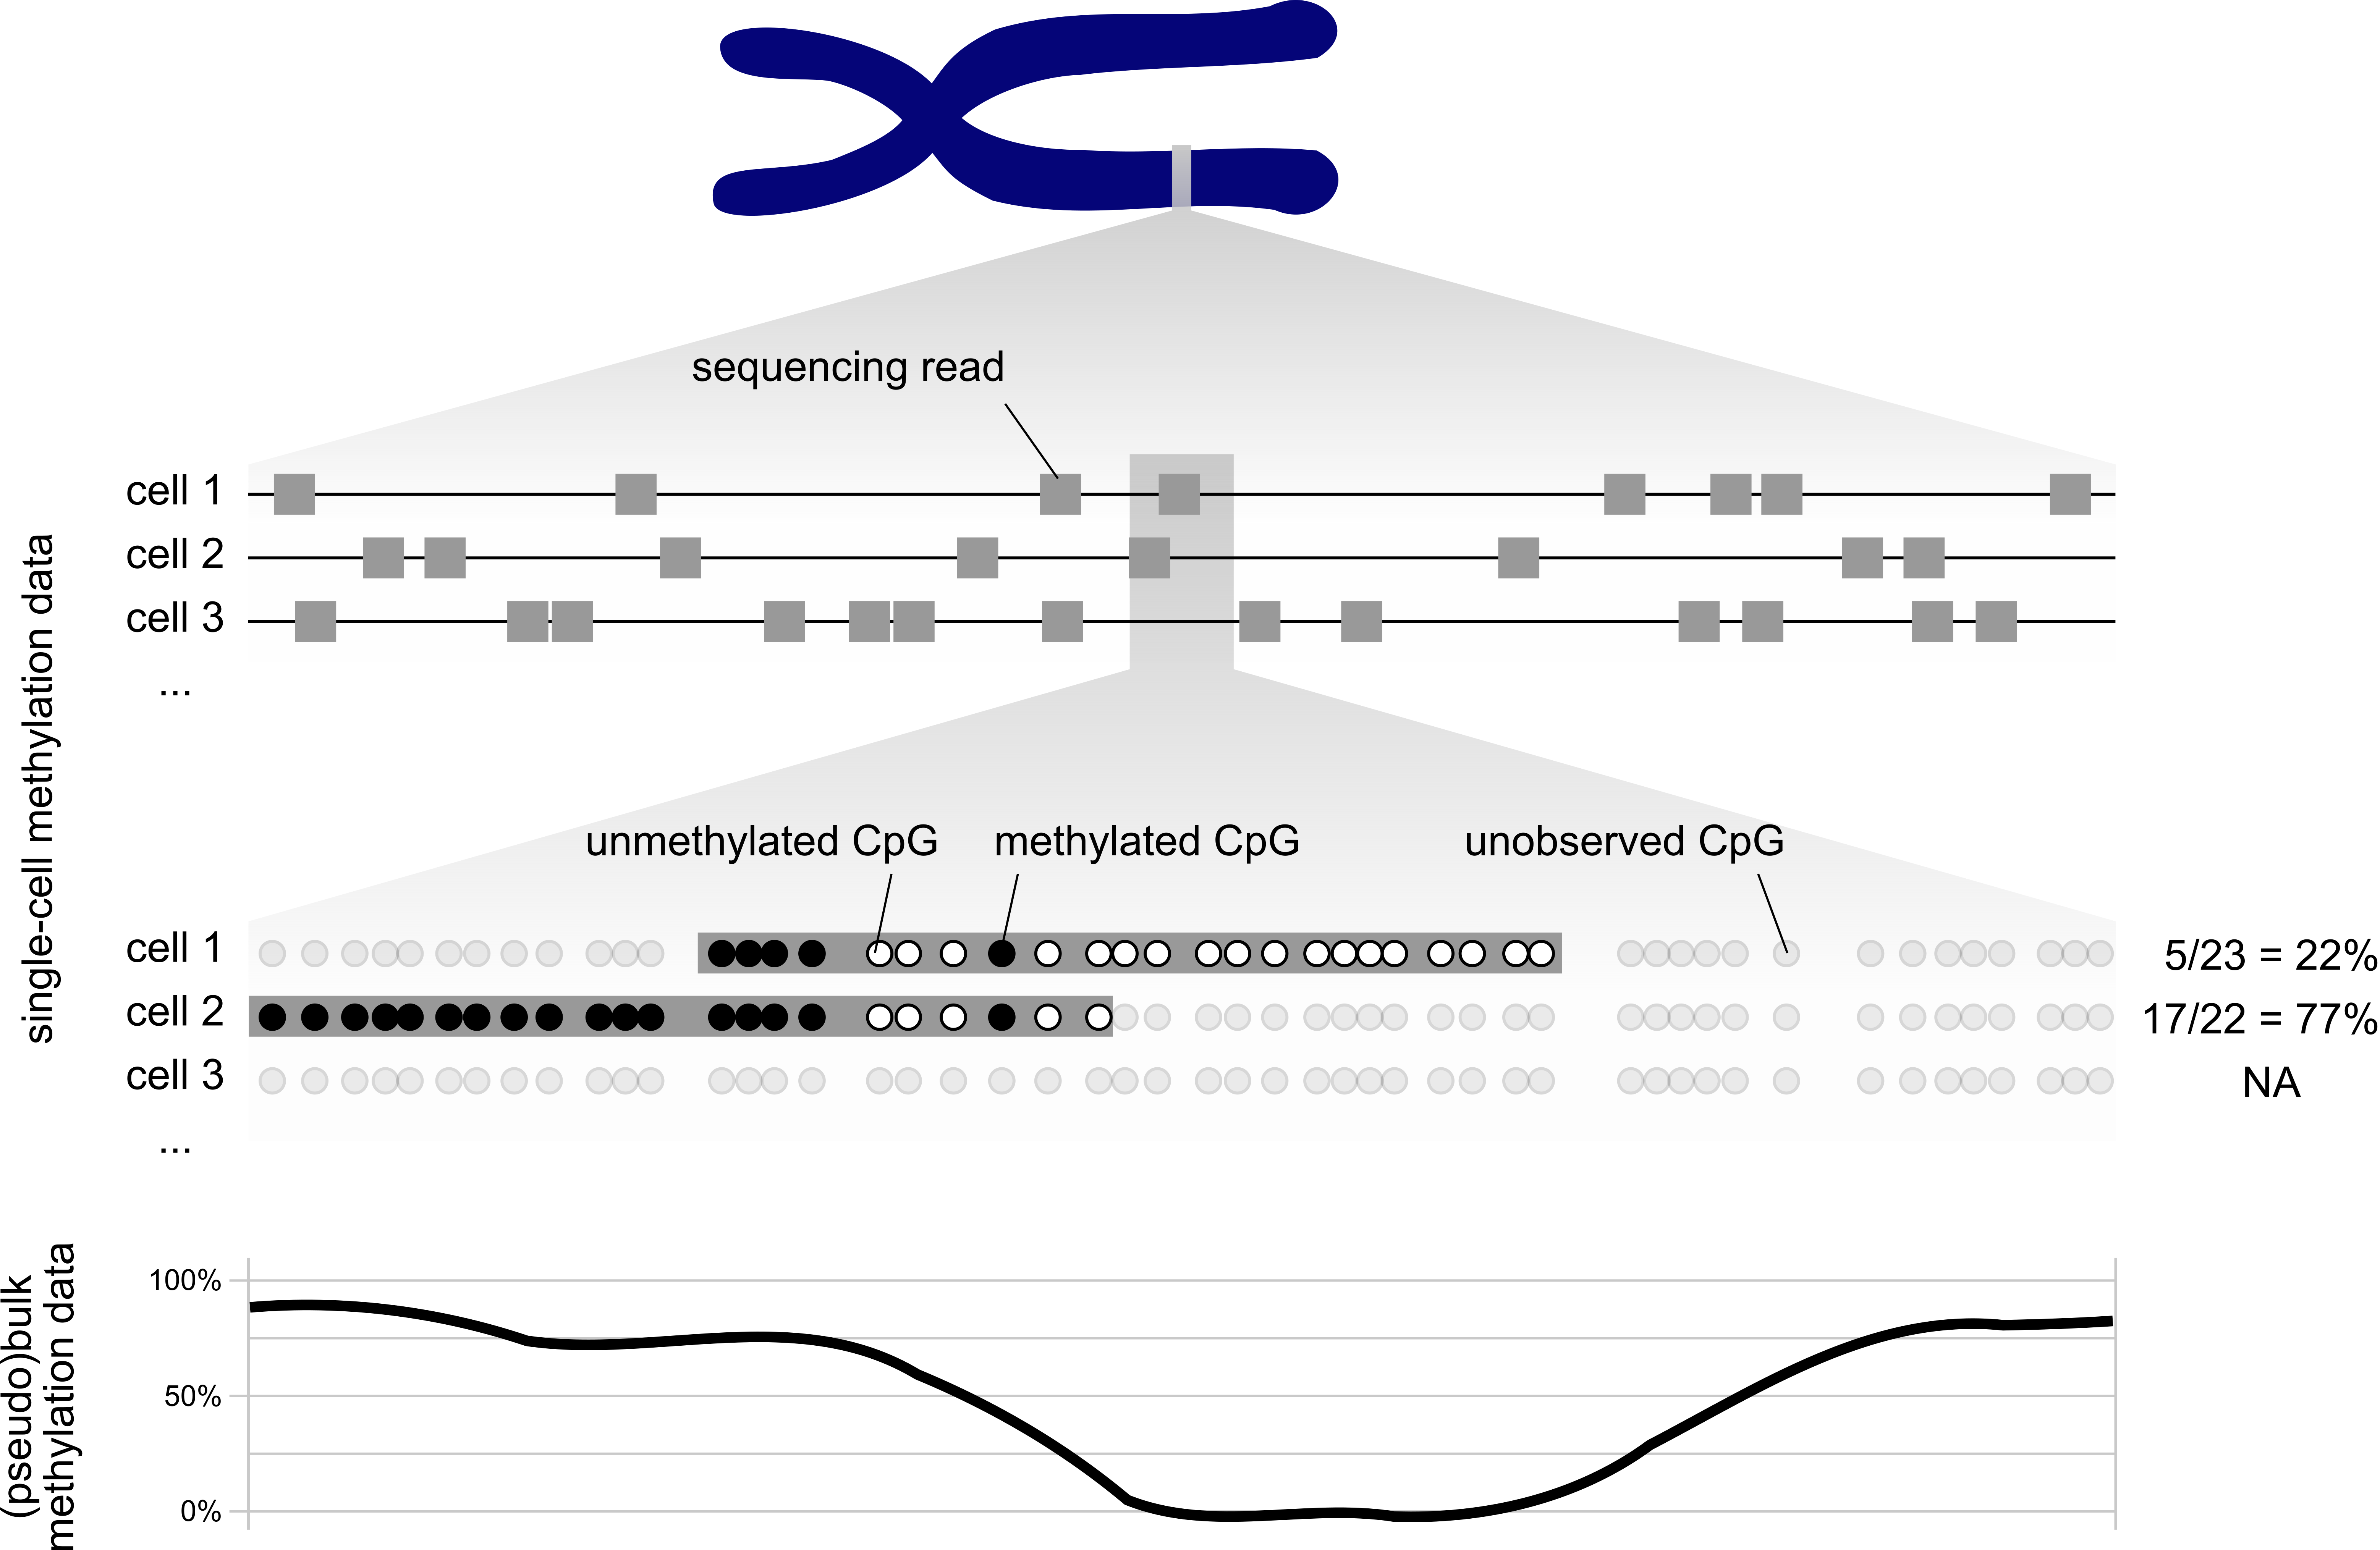
\includegraphics[width=0.75\textwidth]{figures/Fig_residuals_A.png}\\
    \end{center}
	B\\
    \begin{center}
        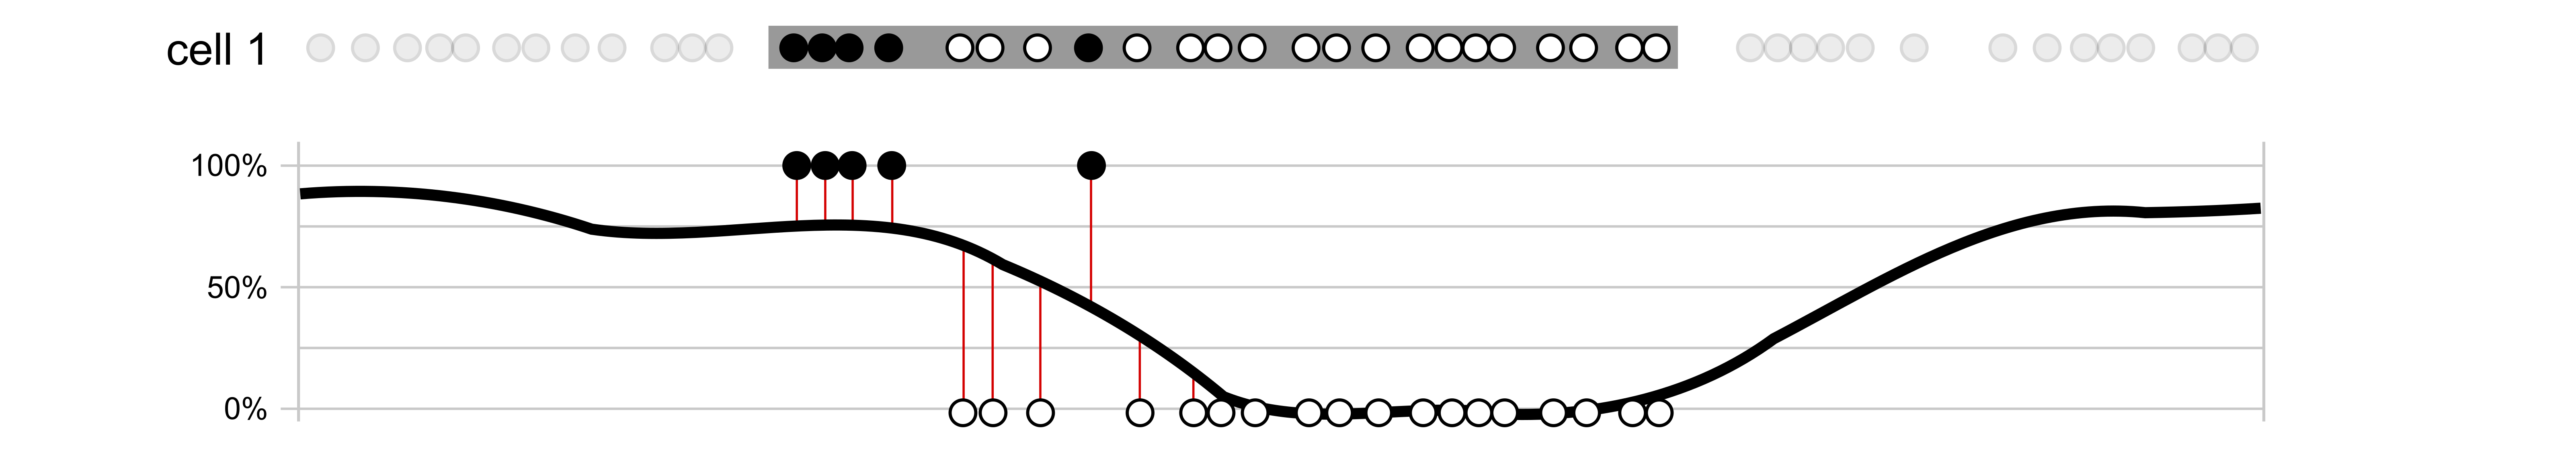
\includegraphics[width=0.75\textwidth]{figures/Fig_residuals_B.png}
    \end{center}
\caption{\small \textbf{Effect of read position:} \textbf{(A)} Depicted is a genomic interval along a chromosome, for which DNA methylation is to be quantified. Two cells cover differing parts of the interval with one read each. If one simply counts for each cell which fraction of the covered CpG sites are methylated, one obtains very different values for the two cells. \textbf{(B)} By averaging each CpG site's methylation over all cells and subsequent smoothing, the thick black ``average methylation curve'' is obtained. To quantify the methylation of cell 1 from (A) relative to this average over all cells, we propose to use the cell's residuals to the smoothed curve (lengths of the vertical red lines) and take their average, counting residuals of methylated CpGs positive and residuals of unmethylated CpGs negative.}
\label{fig:smoothres}
\end{figure*}


\section{Three improvements to processing scBS data}

\subsection{Smoothing residuals} \label{residuals}

We first discuss the task of quantifying the level of methylation in given, fixed, genomic interval. In Figure \ref{fig:smoothres}A, such an interval is covered by a single read for each of the two cells shown. The read from the cell 2 shows much more methylation than the read from cell 1, and a simple analysis would therefore consider that cell as having stronger methylation in the interval. However, given that the two reads agree wherever they overlap, a more parsimonious interpretation would be that the cells do not show difference in methylation within the interval. Rather, both cells, and similarly maybe most other cells, might have stronger methylation in the left third of the interval than in the middle one.

Therefore, we propose to not first obtain, for each CpG position, an average methylation across all cells and, then quantify for each individual cell its deviation from this average. In Figure \ref{fig:smoothres}B, the curved line depicts such an average over all cells, the red vertical lines show an individual cell's deviation from the ensemble average. We take the lengths of the red lines as signed values (``residual''), positive for lines extending upwards from the curve (methylated CpG) and negative for lines extending downwards (unmethylated CpG), and take the average over the residual for all the CpGs in the interval that are covered by reads from this cell. The value thus obtained is what we use to quantify this cell's (relative) methylation in the interval. For a genome tiled into such intervals, we thus obtain a matrix, one row per interval, one column per cell, that can be used for downstream analysis, e.g., as input for a PCA.

The signal to noise ratio in a matrix thus obtained will be much better than in a matrix obtained by simply averaging absolute methylation (0 or 1) over all the cell's covered CpG in a region. The reason for this is that we reduce the variation in situation as the one depicted in Figure \ref{fig:smoothres}A, where absolute methylation might differ strongly even though there is no actual evidence for a difference between the two cells.

How should one obtain the ensemble average (the curved line in Fig.\ \ref{fig:smoothres}B)? A simple approach to get a value for a specific CpG would be to take all cells with read coverage for the CpG and use the fraction of these that show the CpG as methylated. However, especially when only few cells offer coverage, these averages will be very noisy. Therefore, we propose to smoothen using a kernel smoother, i.e., by performing a kernel-weighted average over the CpG site's neighborhood. The kernel bandwidth (i.e., the size of the neighborhood to average over) is a tuning parameter; we got good results with 1000~bp and used this value for the examples presented here.

\subsection{PCA with imputation}

The standard PCA algorithm cannot deal with missing data. Therefore, one would need to make intervals wide enough to ensure that every interval is covered by at least one read for most windows and discard any interval that is not covered by any single cell. Hence, a naive analysis has to resort to a coarse tiling of the genome. To counter this, we propose a simple and straightforward way to deal with missing data in the input matrix to a PCA: In a first iteration, we replace each missing value in the centered input matrix with zero, then run the PCA. Then, these zeroes are replaced by the value predicted by the PCA and the PCA is rerun. Convergence is typically achieved after two to four iterations. For details, see Methods. 

The possibility to perform PCA with missing data allows us to use a shorter and thus more intervals and hence provide the PCA with richer input data.

\subsection{Finding variably methylated regions}

\begin{figure}
	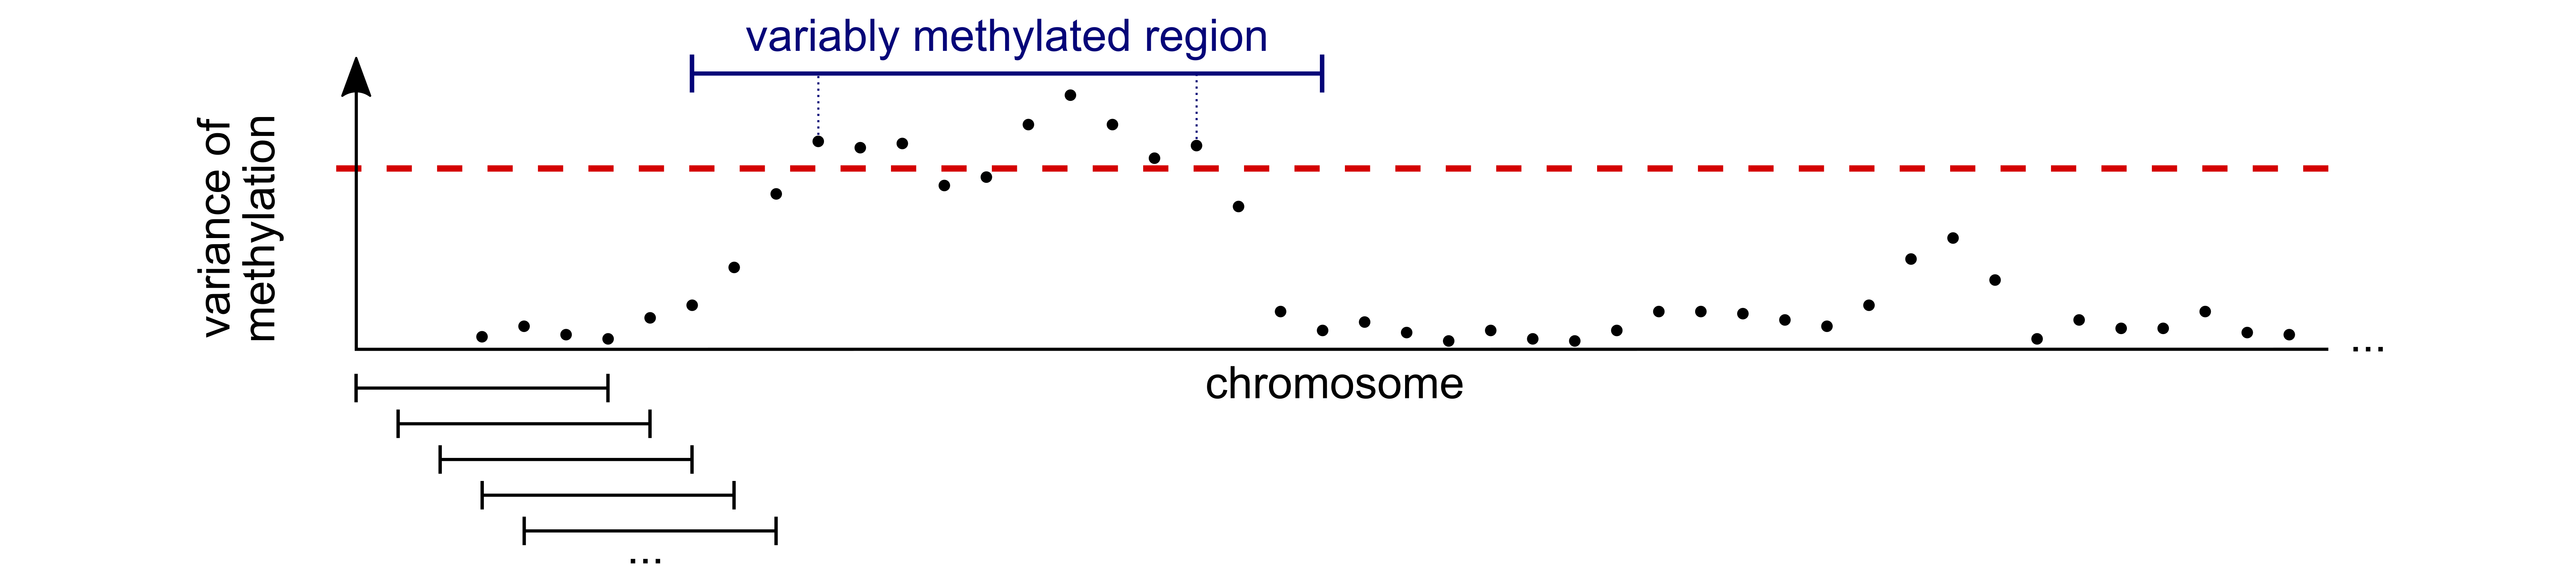
\includegraphics[width=\columnwidth]{figures/Fig_sliding.png}
	\caption{\small \textbf{Finding variably methylated regions (VMR):} The chromosomes are divided up into overlapping windows (first five shown at the bottom), and for each window, the cells' methylation values are calculated as described and as depicted in Fig.\ \ref{fig:smoothres}B. Then, the variance of these values is calculated (each point represents one of the overlapping windows), a threshold (dashed line) is chosen such that a chosen quantile of windows have a variance exceeding the threshold. Windows with above-threshold variance are merged if they overlap, yielding the ``variably methylated regions''.}
	\label{vmr}
\end{figure}


Typically, some regions in a chromosome will have very similar methylation status in all cells (most commonly, fully methylated in nearly all cells) while other regions show variability in methylation across cells. Only the latter regions are of value for our goal of quantitating dissimilarity between cells. We call these the variably methylated regions (VMRs).

So far, we have discussed dividing up (tiling) each chromosome genome into non-overlapping, equal-sized intervals, and quantitating the methylation of each such window. Such rigid placing of interval boundaries is unlikely to be optimal: for example, a VMR might be much smaller than a tile and its signal will hence be drowned out by the larger part of uninformative CpGs that are equal in all cells, when averaging over all the CpG sites in the tile.

Therefore, we propose the following approach (Fig. \ref{vmr}): Divide up the chromosome into many \emph{overlapping} windows, that start at regular multiples of a fixed, small, step size. Quantify the methylation of each cell in each window by averaging the cell's methylation residuals over all CpGs in the window, as described above and depicted in Figure\ \ref{fig:smoothres}B. Then, calculate for each window the variance of these values over all cells. Select, say, the top XX\% windows with the highest variances and mark them as VMRs. Wherever thus marked windows overlap or are divided by only a small gap, merge them into one larger VMR. Then, calculate for each of these larger VMRs the methylation signal, as before, by averaging for each cell over the residuals of all contained CpGs.

In this manner, we obtain a methylation matrix, with one column per cell and one row per VMR, that is, in a sense, richer in information and has better signal-to-noise ratio than the matrix obtained by the simple analysis sketched at the very beginning. As we demonstrate below, a PCA performed on such a matrix provided a distance metric for the cells that contains more information on biological detail than one from a simpler analysis. 

Besides providing better input for the distance calculations, the identified VMRs can also be compared with genomic annotation, thus providing a useful starting point for examining the data with methods from functional genomics.

\section{The scbs Python package}

\begin{figure*}
    \begin{center}
	    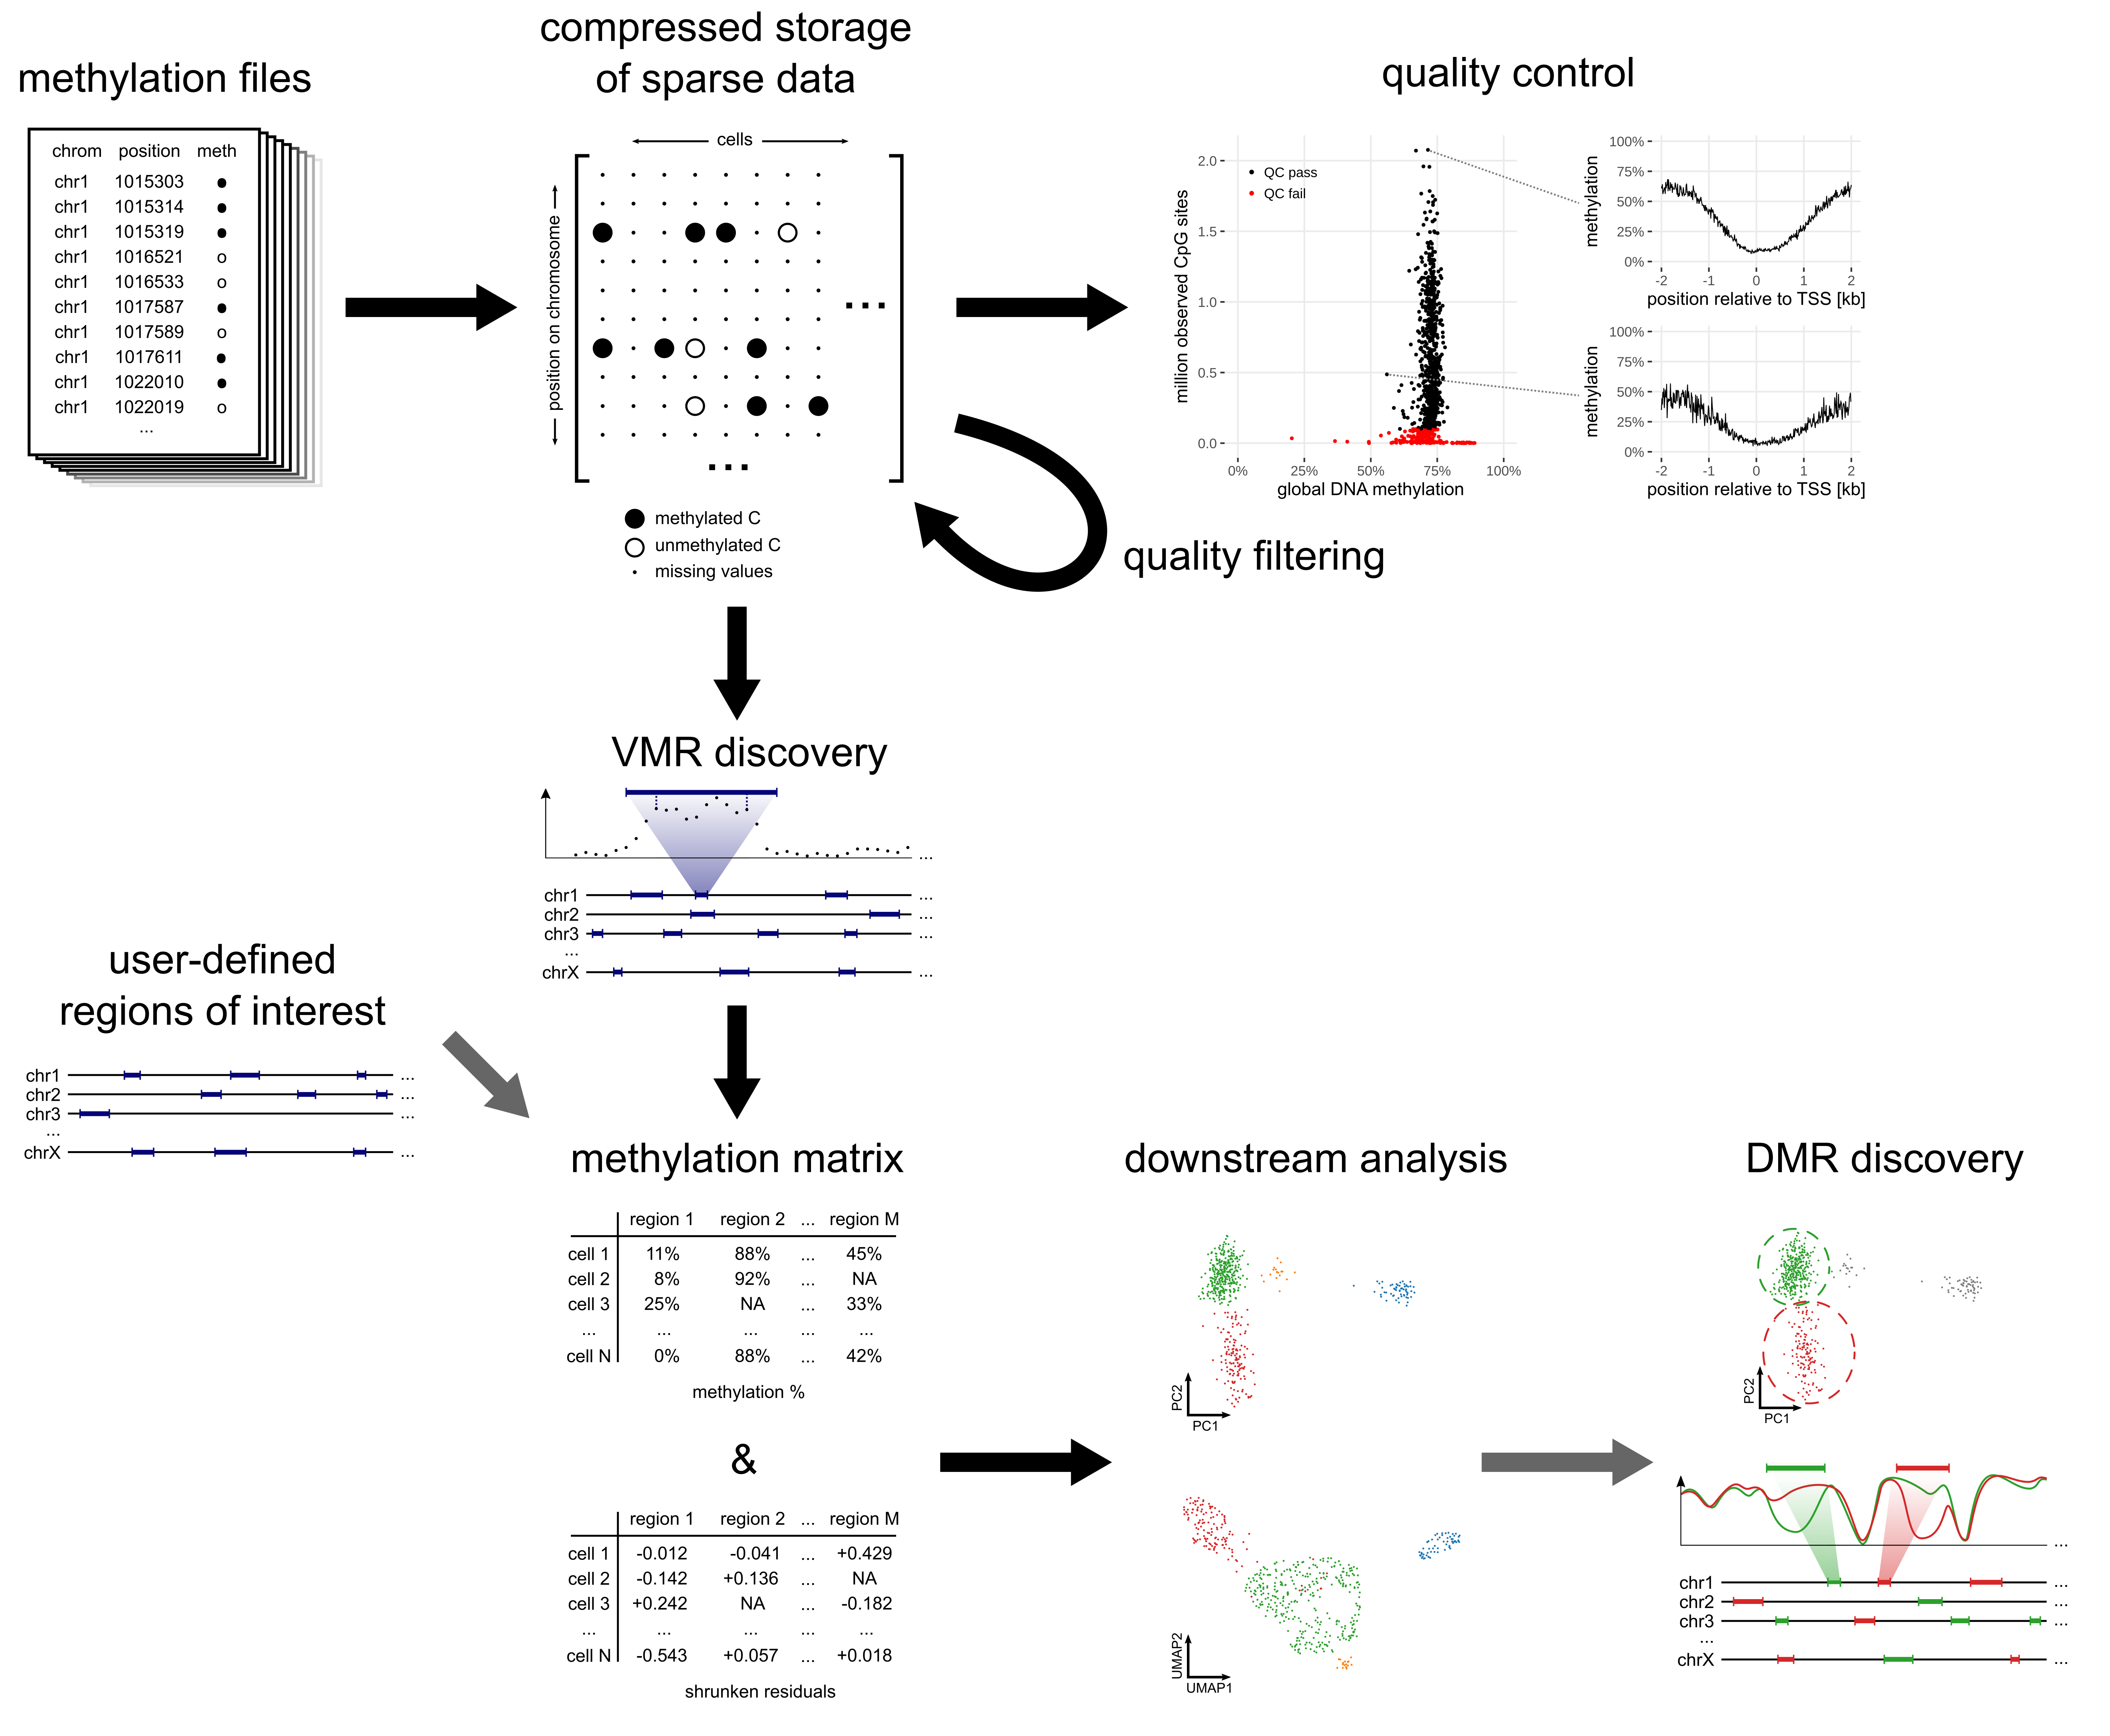
\includegraphics[width=.8\textwidth]{figures/Fig_workflow.png}
    \end{center}
	\caption{\small \textbf{Overview of the functionalities implemented in the scbs package}
	A 
	}
	\label{workflow}
\end{figure*}

We have implemented the approach just described in a Python package with a command line interface, called \texttt{scbs}, which also offers a number of other functionalities for the analysis of scBS data Figure \ref{workflow}. The starting point of such an analysis are methylation files generated by tools such as Bismark \citep{bismark} or methylpy \citep{methylpy}. For each cell, these tools produce a text file that lists the methylation status of all CpG sites. Since it is inconvenient to work with hundreds or thousands of text files, \texttt{scbs} provides the \texttt{prepare} command which parses methylation files and stores their content in a compressed format that enables efficient access to all CpG sites of the genome.

\texttt{scbs prepare} also computes a number of summary statistics for each cell, including the mean genome-wide methylation level and the number of observed CpG sites, i.~e. the number of CpG sites that have sequencing coverage. These summary statistics can be used to detect cells with poor quality. The quality of each single cell methylome can furthermore be inspected with \texttt{scbs profile}, which computes the average methylation profile of a set of user-defined genomic regions such as transcription start sites (TSS). The TSS profile is a useful quality control plot since methylation shows a characteristic dip roughly \textpm1~kb around the transcription start site in mammalian genomes. Cells that do not show this pattern, or cells with few observed CpG sites, may then be filtered from the data set with \texttt{scbs filter}. 

After quality control, the user has access to the previously described genome-wide VMR detection approach via \texttt{scbs scan}. This produces a BED-file that lists the genome coordinates of VMRs. To finally obtain a methylation matrix analogous to an scRNA-seq count matrix, this BED-file can be used as input for \texttt{scbs matrix}, which quantifies methylation at genomic intervals in all cells. The command produces both the percentage of methylated CpG sites, as well as our proposed methylation measure (shrunken mean of the residuals) that is more robust to variation in sequencing coverage or stochastic differences in read position between cells. We note that both \texttt{matrix} and \texttt{profile} accept any valid BED-file as input, which means that the user can quantify and visualize methylation at any genomic feature of interest, such as promoters, enhancers or transcription factor binding sites. The obtained methylation matrix can then serve as input for common single-cell analysis methods such as dimensionality reduction and cell clustering.

\texttt{scbs} is free and open source, and the package can be installed via the Python package manager. The source code and the package are available at \href{https://github.com/LKremer/scbs}{https://github.com/LKremer/scbs}, where we also provide detailed documentation including a tutorial that demonstrates a complete \texttt{scbs} analysis on an example data set.


\section{Comparison}

To demonstrate an improvement of results, we compare previously published analyses described above with our analysis method.
First, we use a data set by \citet{argelaguet2019gastru}. In their work, they generated a single cell methylome data set of mouse embryo cells across different stages of development (E4.5 – E7.5). They calculated the correlation between RNA expression intensity and corresponding DNA methylation at the promoter region to elucidate the implications of the epigenome on RNA expression during development. As promoters, they used DNA regions of \textpm2~kb around transcriptions start sites (TSS). 




--The following paragraph potentially needs to be changed when new plots are made--




In our analysis, we compare correlations between RNA expression intensity and DNA methylation of these promotor regions to correlations between RNA expression intensity and DNA methylation of the closest variable methylation regions that we identified with \texttt{scbs}. In Figure \ref{figure:correlation}, we show that correlation of RNA expression intensity to gene methylation around the TSS \textpm2~kb is less strong compared to the correlation at the closest variable region. This effect can be observed with methylation fractions (Figure \ref{figure:correlation}A) or shrunken residuals (Figure \ref{figure:correlation}B) as data inputs.

\begin{figure}[!htp]
	A\\
	\hspace{.2cm}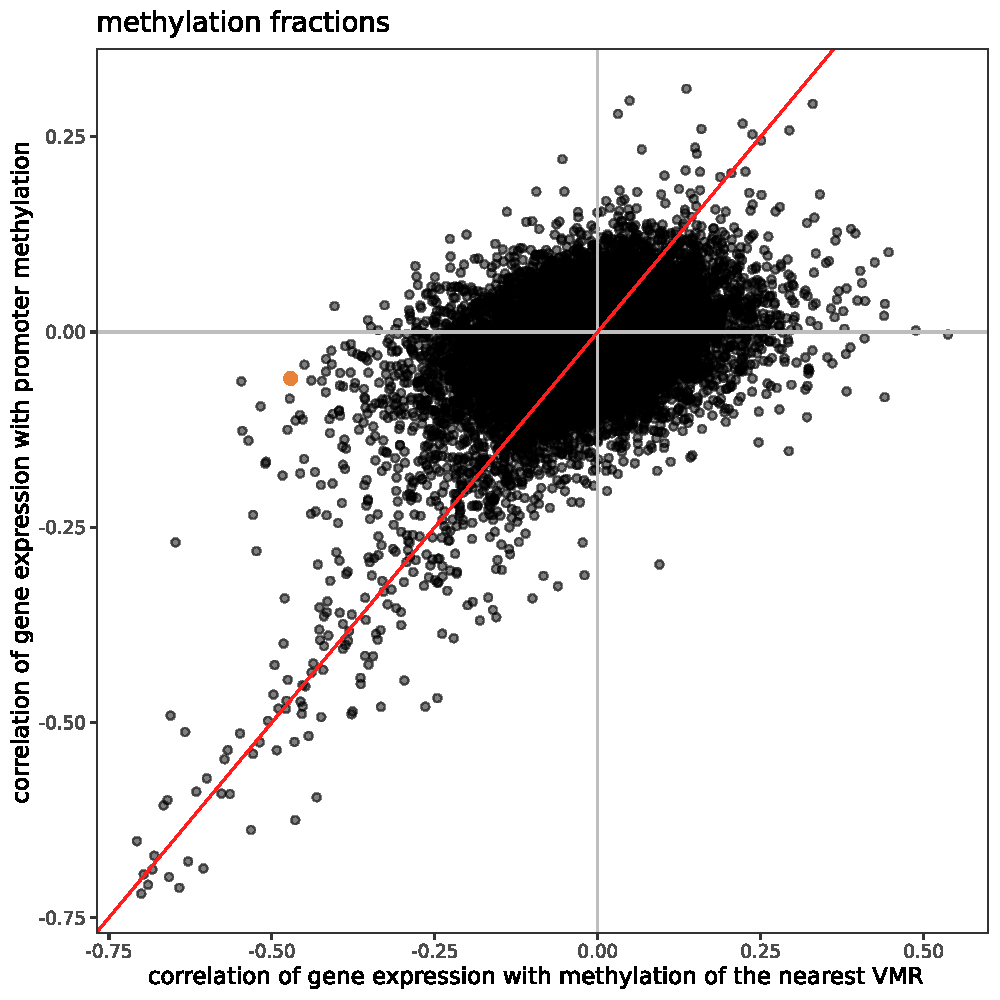
\includegraphics[width=.7\columnwidth]{part_leonie_git/leonie_plots/corr_methylation_fraction_4kbwindow.pdf} \\
	B\\
	\hspace{.2cm}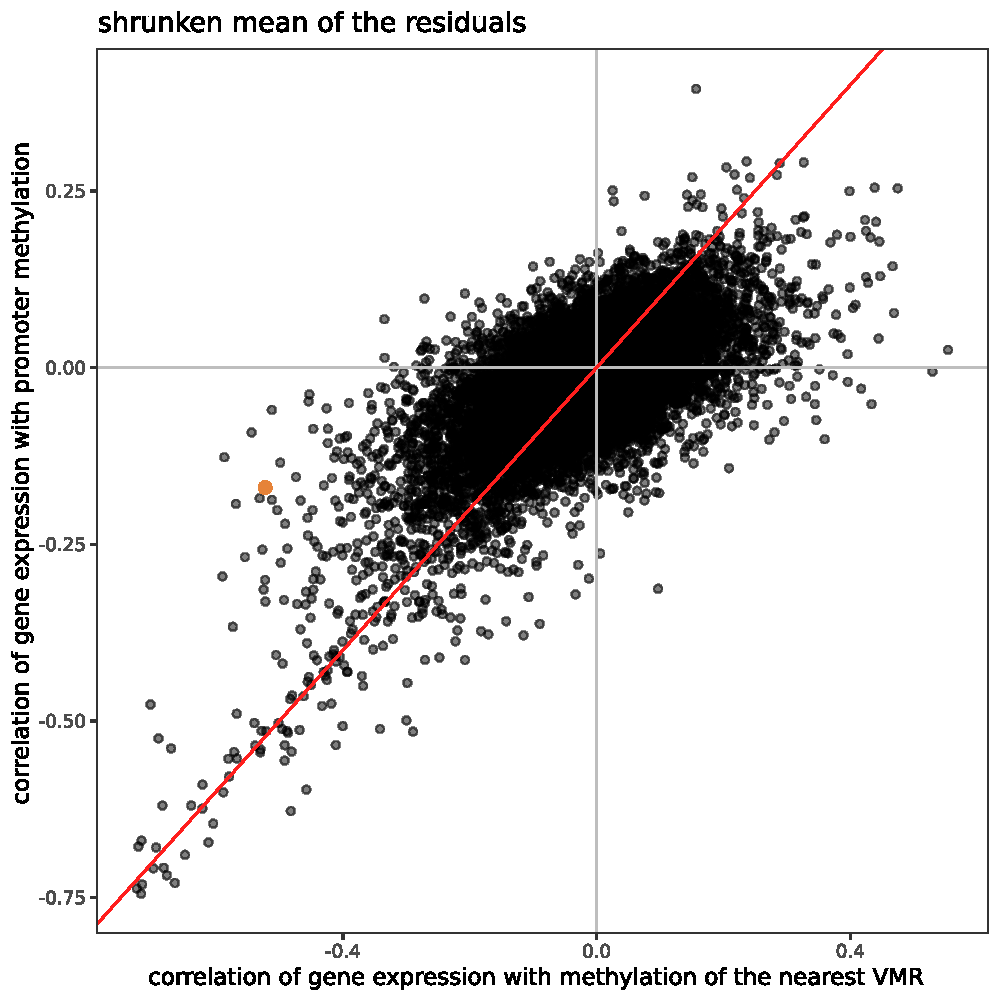
\includegraphics[width=.7\columnwidth]{part_leonie_git/leonie_plots/corr_shrunken_residual_4kbwindow.pdf} \\
	C\\
	\hspace{.39cm}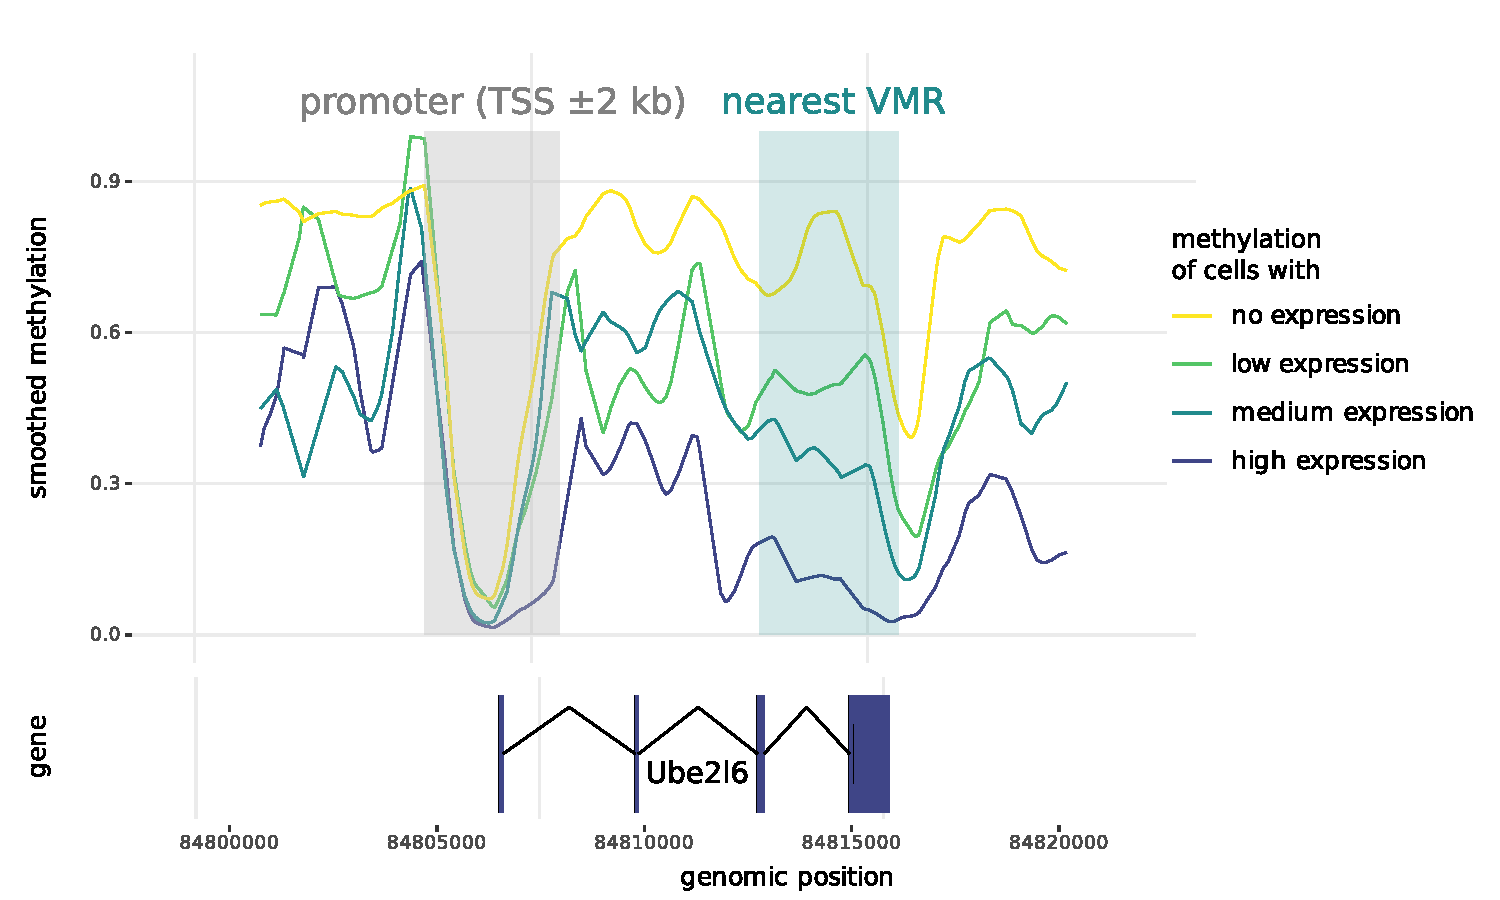
\includegraphics[width=\columnwidth]{part_leonie_git/leonie_plots/comparison_meth_RNA.pdf}

	\caption{\small \textbf{Correlation of DNA methylation and RNA expression intensity}. All plots are based on the data by \citep{luo2017single}.
	\textbf{(A)} Correlation of each gene's RNA expression intensity to methylation fraction of TSS $\pm$ 2kb (y-axis) or to methylation fraction of closest variable gene.
	\textbf{(B)} Correlation of each gene's RNA expression intensity to shrunken residual of methylation of TSS $\pm$ 2kb (y-axis) or to shrunken residual of closest variable gene.
	\textbf{(C)} Mean gene methylation of Ube2l6 gene (ENSMUSG00000027078, marked in yellow in A \& B). Cells were into 4 groups based on their RNA expression (group 0: cells with no expression of gene, group 1-3: cells that express gene divided into three equally large groups with group 3 having the highest expression). Mean methylation level of each group was smoothed with a tricube kernel of bandwidth = 2000.}
	\label{figure:correlation}
\end{figure}

As an example to illustrate this effect more clearly, we picked a gene with significantly stronger correlation at the closest variable region than at the TSS. This gene is marked on Figure \ref{figure:correlation}A and B with a yellow dot. We divided all cells into four groups of cells with no, low, medium and high expression of this exemplary gene Ube216 and plotted a smoothed methylation level per group. As shown in Figure \ref{figure:correlation}C, the promoter region is sparsely methylated in all four RNA expression groups and is therefore a poor region to make conclusions about the relation of DNA methylation and RNA expression intensity. However, a region close to the TSS, identified as the closest highly variable methylation region with scbs, shows a much clearer negative correlation between RNA expression intensity and DNA methylation.  


To further demonstrate the benefit of detecting variable methylation regions, we used a second dataset, published by \citet{luo2017single}. In their work, \citet{luo2017single} generated methylomes from single cell neuronal nuclei in mice to identify genomic regulatory elements across neuron types. To compare how well cell types are separated by different analysis techniques, we processed the same dataset into 2-dimensional UMAPs several times. Subsequently, we compared the results by assigning a score to each output based on cell type separation in the final 15 principal components. We see an improvement of cell separation when comparing the analysis of variable methylation regions to 100 kb regions (\ref{figure:score}A and C). The difference of using shrunken residuals instead of methylation fractions to assess the methylation per region is not as significant. However, when emulating a sparse dataset with less cells by randomly reducing the dataset to 500 cells, it becomes clear that using shrunken residuals over methylation fractions also improves the outcome of our analysis (\ref{figure:score}B and D). 


\begin{figure}[!htp]
	A\\
	\hspace{.3cm}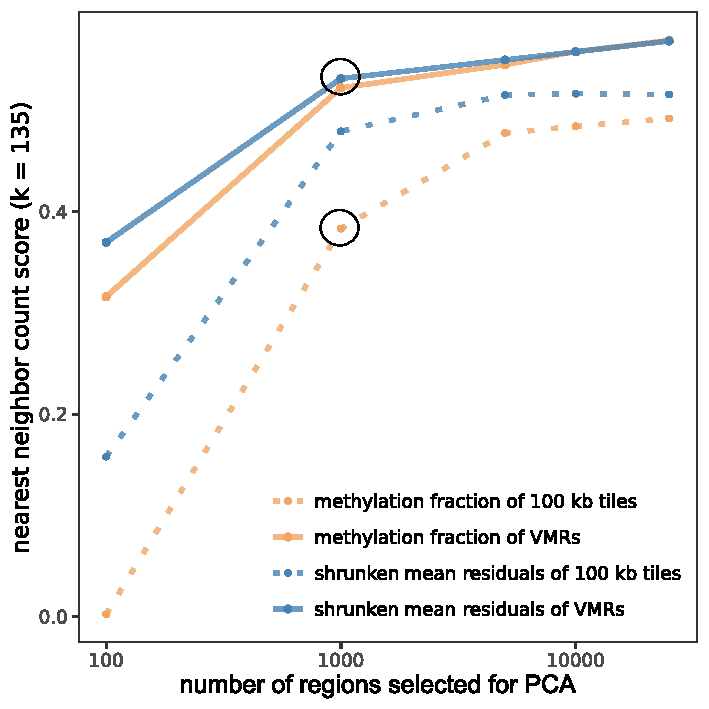
\includegraphics[width=.45\columnwidth]{part_leonie_git/leonie_plots/complete_135k_12cm_log.pdf} 
	B
	\hspace{.3cm}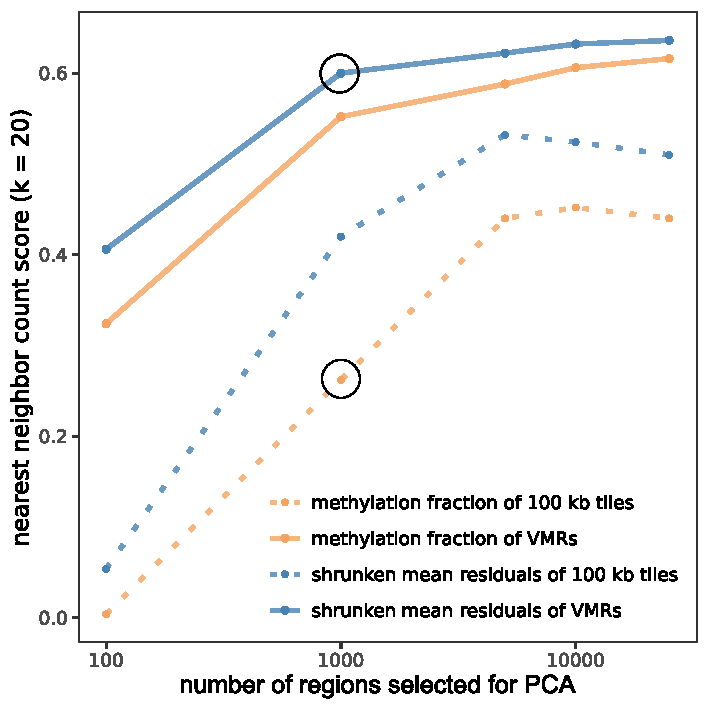
\includegraphics[width=.45\columnwidth]{part_leonie_git/leonie_plots/cell500_20k_12cm_log.pdf} \\
	C\\
	\hspace{.39cm}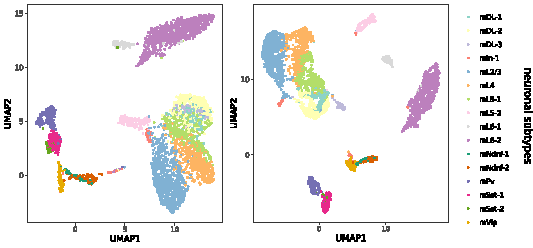
\includegraphics[width=\columnwidth]{part_leonie_git/leonie_plots/UMAP_fulldataset.pdf}
	D\\
	\hspace{.39cm}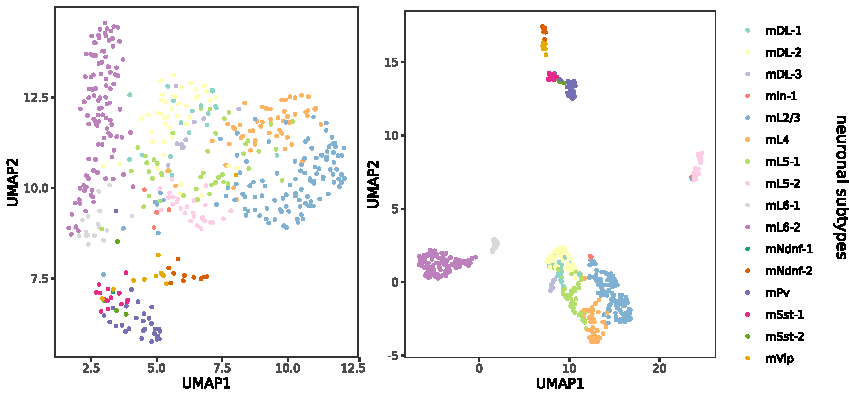
\includegraphics[width=\columnwidth]{part_leonie_git/leonie_plots/UMAP_reduceddataset.pdf}
	\caption{\small \textbf{Analysis comparison}. All plots are based on the data by \citep{luo2017single}. \textbf{(A)} Nearest neighbor count score for complete dataset using four different analysis techniques and a variable number of regions as input. Exemplary UMAPs for encircled scores are shown in (C). \textbf{(B)} Nearest neighbor count score for the same dataset reduced to 500 cells using four different analysis techniques and a variable number of regions as input. Exemplary UMAPs for encircled scores are shown in (D). \textbf{(C)} Two exemplary UMAPs using 1000 regions of the full dataset and methylation fraction of 100 kb windows (left) or shrunken residuals of variable methylation regions (right) \textbf{(D)} Two exemplary UMAPs using 1000 regions of the reduced dataset and methylation fraction of 100 kb windows (left) or shrunken residuals of variable methylation regions (right).}
	\label{figure:score}
\end{figure}

\section{Discussion and Conclusion}

...


\section{Methods}

\subsection{Raw data}

We write $x_{ij}$ for the methylation status of CpG $i$ in cell $j$. The index $i$ runs over all CpG positions present in the genome, the index $j$ over all cells in the assay. We write $x_{ij}=0$ if position $i$ was found to be unmethylated in cell $j$ by bisulfite sequencing , $x_{ij}=1$ if it was methylated, and $x_{ij}=\text{NA}$ if position $i$ was not covered by reads from cell $j$ and the methylation status is therefore not available ("NA"),

These values can be readily obtained from single-cell bisulfite sequencing data using tools like Bismark.

If multiple reads with the same cell barcode cover the positions, these will typically be PCR duplicates of each other and hence agree. Of course, the two alleles of a CpG may differ in their methylation status and while it is in principle possible that one obtains reads stemming the same position on both the paternal and the maternal chromosomes of the same cell, but this is so unlikely that we can ignore the case. Hence, whenever Bismarck reports multiple reads covering the same position in the same cell, we set $x_{ij}$ to 0 or 1 following the majority of reads and put $x_{ij}=\text{NA}$ in case of a tie. 

For later use: We write $C$ for the set of all cells in the assay (i.e., $C$ is the index set for the cell indices $j$). Moreover,
we define $C_i\subset C$ as the set of all those cells $j$ that have reads covering position $i$,
$$ C_i=\{j\in C: x_{ij}\neq\text{NA}\}.$$
Conversely, we define $G_j$ as the set of all the CpG positions $i$ covered by reads from cell $j$ 
$$ G_j=\{i: x_{ij}\neq\text{NA}\}.$$

\subsection{Data preparation}

The function `scbs prepare` reads a set of CpG coverage files (e.g. produced by Bismark) and produces a file that stores the matrix $x$ in a space-efficient format, as follows: $x$ is represented as a SciPy sparse matrix, encoding the actual values 0, 1, and NA as -1, 1, and 0, respectively. Coding NA (the most common value) as 0 leverages SciPy's sparse matrix storage. In all the follows here, any mention of $x$ will, however, always mean the encoding as $x_{ij}\in\{0,1,\text{NA}\}$.

\subsection{Smoothing}

For each CpG position $i$, we write 
$$\overline{x}_i=\langle x_{ij} \rangle_{j\in C_i} = \frac{1}{|C_i|}\sum_{j\in C_i} x_{ij}$$ 
for the average methylation at position $i$, where $\langle\cdot\rangle$ denotes averaging, and the average runs over all the cells $i\in C_j$, i.e. over those cells for which methylation data is available for position $i$.

NOTE: Here, we could already do shrinkage and use $\frac{1}{|C_i|+1}\sum_i x_{ij}$ intead. But we don't do that, right?

We then run a kernel smoother over these per-position averages to obtain the smoothed averages $\tilde x_i$. Specifically, we use

\[ \tilde x_i = \frac{\sum_{i'} \overline x_{i'}\, k_h(d_{ii'})}{\sum_{i'} k_h(d_{ii'})},\]
i.e., $\tilde x_i$ is the weighted average over the per-position averages $\overline{x}_{i'}$, taken over the CpG sites $i'$ in the neighborhood of $i$, and weighted using a smoothing kernel $k_h$ with bandwidth $h$. Here, $d_{ii'}$ is the distance between CpG positions $i$ and $i'$, measured in base pairs, $h$ is the smoothing bandwidth in base pairs (by default, $h=1000$), and $k_h$ is the tricube kernel,

\[ k_h(d) = \left\{
\begin{aligned}
	&\left(1-|d/h|^3\right)^3 &\text{for } |d|<h \\
	&\,0 &\text{otherwise}. 
\end{aligned}
\right.
\]

We also provide Here, we could weight the positions by number of covered cells, i.e., use

$$ \tilde x_i = \frac{\sum_{i'} \overline x_{i'}\, k_h(d_{ii'})\, n_{i'}}{\sum_{i'} k_h(d_{ii'})\, n_{i'}},$$

but we don't do that, or do we?


\subsection{Methylation for an interval}

Next, we discuss averaging methylation over a range of CpG sites.

Given an interval $I$ on the chromosome, we wish to quantify the average methylation $m_{Ij}$ of the CpG sites within the interval for cell $j$. If we interpret $I$ as the set of CpG positions $i$ in the interval, we may write

$$ m_{Ij} = \left< x_{ij} \right>_{i\in I\cap G_j}.$$

Here, the average runs over all those sites $i$ that lie within the interval $I$ and are covered by reads from cell $j$.

If we wish to compare cells, it can be helpful to center this quantity by subtracting its average:

$$ z_{Ij} = m_{Ij} - \langle m_{Ij'}\rangle_{j'\in C}.$$

As an alternative, we suggest to consider the residuals of the individual CpG methylation values $x_{ij}$ from the smoothed average $\tilde x_i$,
$$ r_{ij} = x_{ij} - \tilde x_i, $$
and averaging over these, obtaining
\begin{equation} 
r_{Ij} = \frac{\scriptsize{1}}{\scriptsize{|I\cap C_i|+1}}\sum_{i\in I\cap C_i}\left( x_{ij} - \tilde x_i \right). \label{avgres}
\end{equation}

This is a shrunken average, with denominator $n+1$. This extra pseudocount has the effect of shrinking the value towards the "neutral" value 0, with the shrinkage becoming stronger if the data is "weak" because the number $|I\cap C_i|$ of positions covered by reads from cell $j$  is low. In the extreme case of none of the reads from cell $j$ covering $I$, the sum becomes 0 and the denominator 1, i.e. $r_{Ij}=0$ in this case.

\subsection{Finding variably methylated regions (VMRs)}

For any interval $I$, we denote by $v_I$ the variance of its residual averages $r_{Ij}$:

$$ v_I = \frac{\scriptsize{1}}{\scriptsize{|C_I|}}\left( r_{Ij} - \langle r_{Ij'}\rangle_{j'\in C_I} \right)^2,$$

where the average runs only over the set $C_I=\bigcup_{i\in I}C_i$ of those cells $j$ which have reads covering interval I.

To find VMRs, we define intervals $I_1, I_2, ...$, all of the same width, and with step-wise increasing starts, then calculate $v_1, v_2, ...$ for these intervals. We then mark the intervals with the 2\% highest variances. We take the union of all these intervals, split the union into connected components, and call each component a VMR. Putting that last step in other words: We take all the intervals with variance in the top 2-percentile, fuse intervals that overlap and call the regions thus obtained the VMRs.

\subsection{Calculating cell to cell distances}

Given a set, $\mathcal{V}=\{I^\text{v}_1,I^\text{v}_2,\dots\}$, of intervals corresponding to VMRs, we get a relative methylation fraction $r_{ij}$ for each VMR $I^\text{v}_i$ and each cell $j$ from Eq.\ ()\ref{avgres}). The matrix thus obtained can then be centered and used as input for a PCA. If we calculate the top $R$ principal components, we thus obtain for each cell $j$ an $R$-dimensional principal component vector $\mathbf{x}^\text{P}_j$. For any two cells $j$, $j'$, we use the Euclidean distance $\|\mathbf{x}^\text{P}_j - \mathbf{x}^\text{P}_{j'}\|$ as the measure of dissimilarity of the two cells. Thus, the matrix of PC scores can be used as input to dimension reduction methods like t-SNE or UMAP, and to clustering methods like the Louvain or Leiden algorithm, which requirte such a matrix as input to the approximate mnearest neighbor (ANN) finding algorithm that is their first step.

\subsection{PCA with imputation}

[...]


{\small \bibliography{scbs}}

\end{document}